\documentclass[a4paper,10pt]{article}
\usepackage[utf8]{inputenc}
\usepackage{frontespizio}
\usepackage{listings}
\usepackage{pdfpages}
\usepackage[usenames,dvipsnames]{color}

\definecolor{codegreen}{rgb}{0,0.6,0}
\definecolor{codegray}{rgb}{0.5,0.5,0.5}
\definecolor{codepurple}{rgb}{0.58,0,0.82}
\definecolor{backcolour}{rgb}{0.95,0.95,0.92}

\lstdefinestyle{mystyle}{
    backgroundcolor=\color{backcolour},   
    commentstyle=\color{codegreen},
    keywordstyle=\color{magenta},
    numberstyle=\tiny\color{codegray},
    stringstyle=\color{codepurple},
    basicstyle=\footnotesize,
    breakatwhitespace=false,         
    breaklines=true,                 
    captionpos=b,                    
    keepspaces=true,                 
    numbers=left,                    
    numbersep=5pt,                  
    showspaces=false,                
    showstringspaces=false,
    showtabs=false,                  
    tabsize=2
}
\lstset{style=mystyle}

% Title Page
\title{Relazione progetto di Basi di Dati}
\author{Giovanni Liboni}


\begin{document}
\begin{frontespizio}

\Universita{Verona}
\Dipartimento{Informatica}
\Corso[Laurea]{Informatica}
\Titoletto{Consegna G4 - Sistema informativo per la gestione dell'emissione di biglietti aerei}
\Titolo{Relazione finale del progetto di Basi di Dati }

\Candidato[VR363021]{Giovanni Liboni}

\Annoaccademico{2013-2014}
\end{frontespizio}

\tableofcontents

\newpage

\part{Progetto della basi di dati}

\section{Progetto concettuale}
Qui di seguito si riporta il diagramma Entit\`a - Relazione e lo schema concettuale ricavati dalle specifiche del progetto.
A partire da questo schema si sono scritte le tabelle per la Base di Dati.

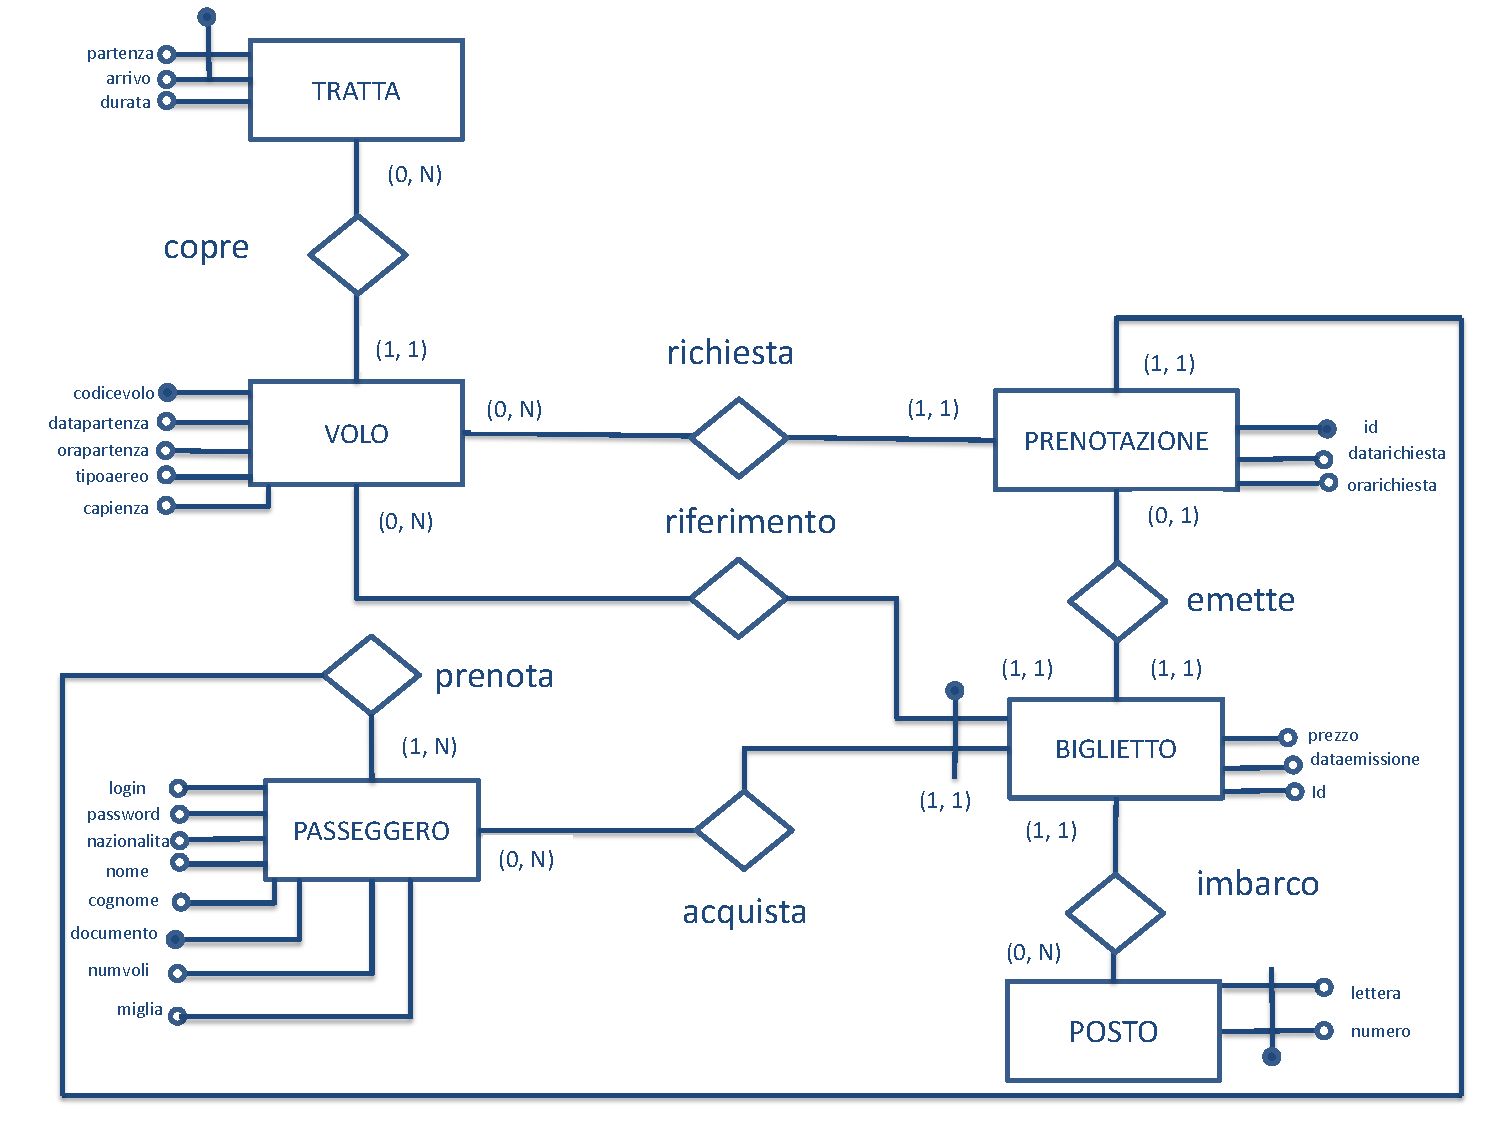
\includegraphics[scale=0.5]{er.pdf}

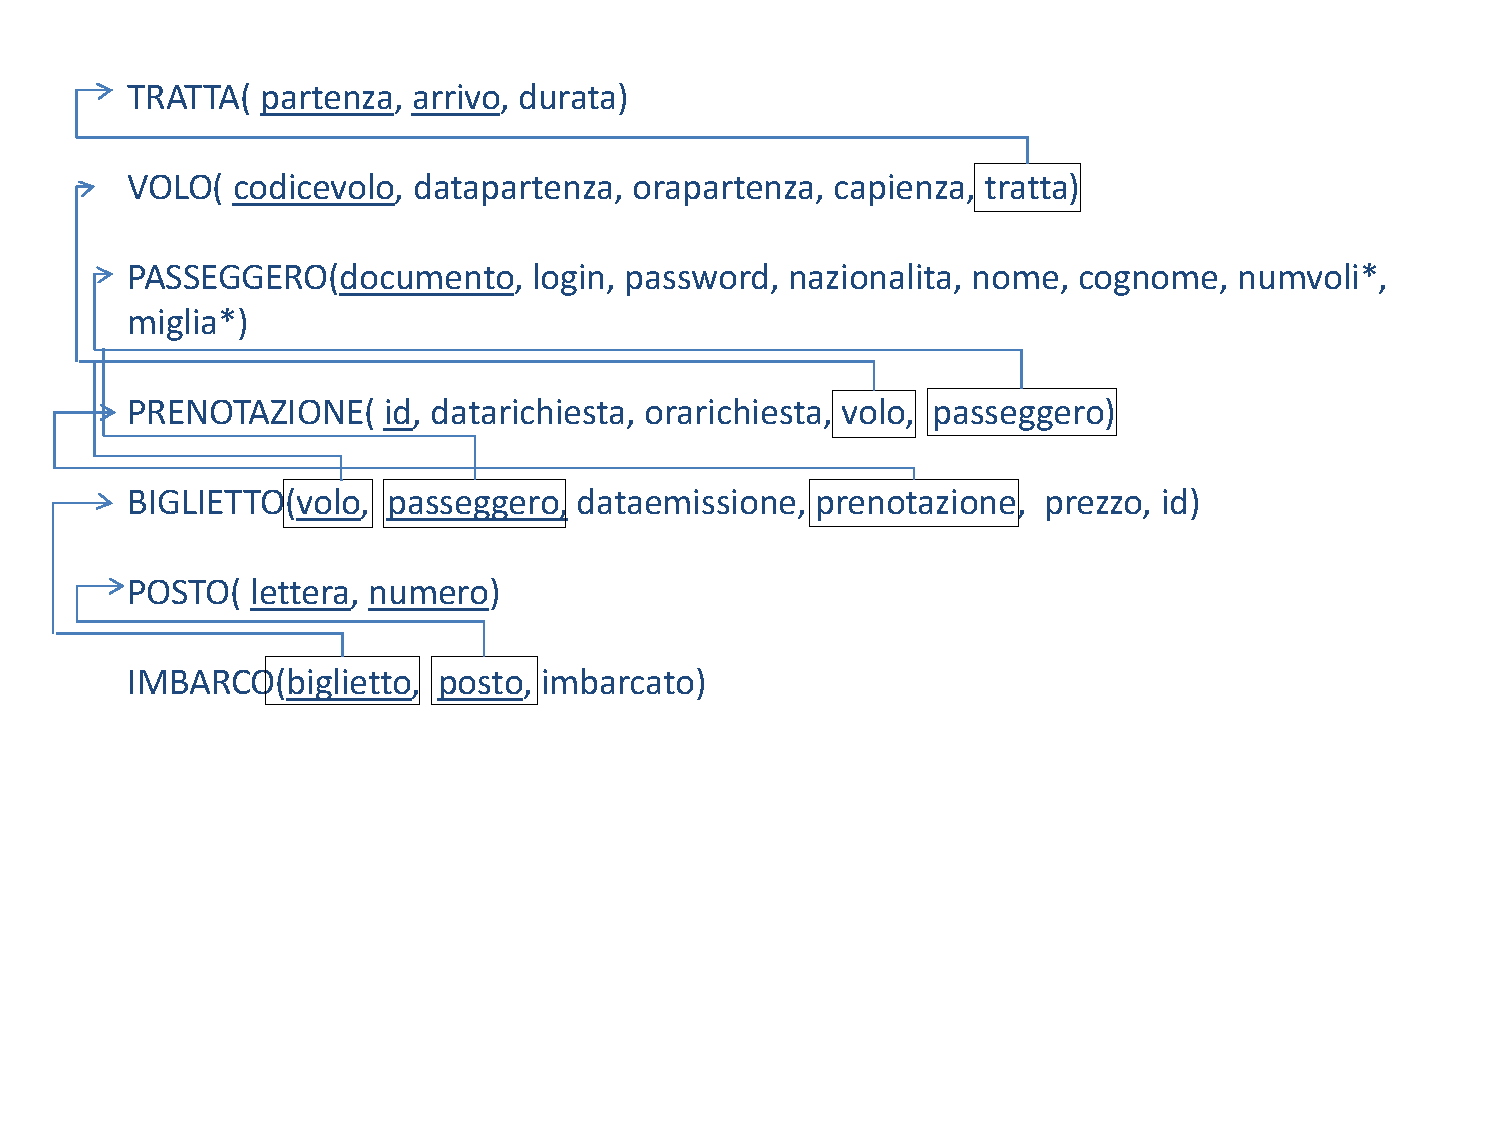
\includegraphics[scale=0.6]{schemalogico.pdf}

Descrivere il diagramma e lo schema logico.

\section{Progetto logico}

Abbiamo usato un singolo script per la creazione delle tabelle sul database. Il codice viene riportato qui di seguito.

\lstinputlisting[language=SQL]{create_table.sql}

Abbiamo aggiunto delle funzioni scritte in \textit{plpgsql} per eseguire azioni di routine sul base di dati e per inserire automaticamente la data e l'ora di inserimento di determinate tuple.
Si riporta di seguito il codice delle funzioni create.
\lstinputlisting[language=SQL]{create_function.sql}

Per automatizzare l'esecuzione delle funzioni si sono scritti dei trigger, azioni eseguite al verificarsi di certe condizioni. I trigger creati sono i seguenti:
\lstinputlisting[language=SQL]{create_trigger.sql}

\section{Popolamento della base di dati}

\part{Progetto del sito web}

\section{Progettazione logica}

Si riportano di seguiti gli schemi di pagina seguiti durante la creazione del sito.

\section{Struttura dell'applicazione web}

\part{Architettura MVC2}
L'elaborato \`e stato sviluppato seguendo il design pattern MVC2 e seguendo l'approccio servlet-centric. Questo pattern \`e composto da tre moduli:

\begin{itemize}
 \item Model - Comprende la classe DBMS.java e i Java Data Beans. I beans sono contenuti nel package \textit{bean}, mentre la classe DBMS.java \`e contenuta nel package \textit{database};
 \item View - Comprende tutte le JSPs, i javascript e i css;
 \item Controller - Comprende le servlet main.java, picture.java.  Ogni servlet ha un compito specifico: ... ;
\end{itemize}

\part{Model}
Fanno parte del modulo Model il DBMS e i javabeans. 
\part{View}
Fanno parte del modulo View tutte la JSPs, i javascript e i css.
\part{Controller}
Fanno parte del modulo Controller le due servlet. Le due servlet che controllano il flusso sono \textit{main.java} e \textit{picture.java}. 

La servlet \textit{picture.java} gestisce la parte multimediale dell'applicazione, caricando e scaricando dalla base di dati le foto profilo dei passeggeri.
Per ogni richiesta viene passato il parametro \textit{ps} con un determinato valore e pu\`o assumere questi valori:
\begin{itemize}
 \item uploadimage
 \item downloadimage
\end{itemize}

La servlet \textit{main.java} controlla le richieste da parte delle JSPs.

\begin{itemize}
 \item areapersonale - Vengono caricati dalla base di dati i voli e le prenotazioni dell'utente specificato nel parametro \textit{pass}.
 \item ricercavolo 
 \item volipage
 \item prenotazione
 \item nuovaprenotazione
 \item logout
 \item login
 \item contatti
 \item emettibiglietto
 \item newbiglietto
 \item chisiamo
 \item ajaxricercavolo
 \item checkusername
 \item checkdocumento
\end{itemize}

\part{Scelte progettuali}

\section{Hibernate}
\section{AJAX}
\section{Session}

\end{document}          
